%To evaluate the behavior and accuracy of ConPaaS when hosting web applications, we prepared a realistic and complex enough scenario to assess any PaaS. In particular, we deployed the Wikipedia web application called MediaWiki~\cite{mediawiki}, and used a web hosting benchmark called WikiBench~\cite{wikibench}. 

%1. The heterogenity of the requests of wikipedia and realistic scenario.

Most academic resource provisioning systems are evaluated using
synthetic applications and workloads such as TPC-W, RuBiS and
RuBBoS. However, these traditional benchmarks do not exhibit features
of real Web applications such as traffic unstability as well as
heterogeneous and constantly-changing request mixes~\cite{benchlab}.

Instead of basing our evaluations on unrealistic workloads, we used
the WikiBench benchmark~\cite{wikibench}. This benchmark uses a full
copy of Wikipedia as the web application, and replays a fraction of
the actual Wikipedia's access traces. 


%Wikipedia uses
%MediaWiki~\cite{mediawiki}, a PHP-based wiki software package.
%The architecture of the Wikipedia website uses a http-proxy, a http-web server, a database and one or more PhP servers. 
Hosting a copy of Wikipedia in ConPaaS requires two different
services: a PHP web hosting and a MySQL service. The MySQL service is
loaded with a full copy of the English Wikipedia articles as of 2011,
which has a size of approximately 40GB.  In the PHP service, the
configuration was composed of one load balancer, one or more static web server
and one or more PHP servers. We then use WikiBench to replay access
traces from 2011~\cite{urdaneta2009}.



%ConPaaS uses nginx as static web server and also as load balancer.% The PHP requests are handled through PHP FastCGI Process Manager.
%In the PhP service, an initial configuration was composed of one Nginx http-proxy, one Apache server, and one or more PhP (FastCGI Process Manager) servers. Each PhP server hosts the MediaWiki application which is the main component of this system. 

% 3. Presentation of the preeliminary experiment

%To evaluate our system we used Wikibench, a tool for
%benchmarking Wikipedia servers developed by our group. Wikibench
%replays Wikipedia access traces or smaller samples of the traces,
%providing various sampling mechanisms.
%We used anonymized Wikipedia access traces, which are published by the WikiMedia foundation, and for our experiments we replayed a sample of 10\% from the traces. 
The trace contains requests for static pages as well as dynamic PHP
requests. When replaying it, the most important performance bottleneck
is the application logic of the application: PHP requests are
processed an order of magnitude slower than simpler static web
pages. In this article we therefore focus on the automatic scaling of
the PHP tier.

As an example, in Figure~\ref{workload}, we show the PHP workload
sampled from one trace, as the number of PHP requests per minute
during approximately one day. One aspect that we noticed about the
workload is that the requests are heterogeneous in complexity.  To
illustrate this heterogeneity, in Figure~\ref{phpRespTimeDispersion}
we present the distribution of the response time values for the PHP
requests during the execution of the trace shown in
Figure~\ref{workload}.  For this experiment we used a fixed number of
one web server (1-core 2.4Ghz and 1Gb RAM) and three PHP servers (8-core 2.4Ghz and 8Gb RAM), which are sufficient for handling the workload from the
access trace even at its peaks; this is why in this case the response
time is not influenced by the intensity of the workload.  However, the
results show a relatively wide dispersion of the response time: the
response time values are commonly spread between approximately 100 and
300 milliseconds, so there is a factor of 3 between the slowest and
the fastest requests.  The main reason for this dispersion is that the
Wikipedia articles vary in complexity, requiring different amounts of
information that needs to be retrieved from the database and assembled
in a page.

% 4. Expectations for the evaluation presented

We also conclude from this experiment that, since the response time of
the application varies and cannot be properly predicted even when the
request rate is known, a provisioning algorithm aiming to keep the
application's response time under a certain limit should take into
account several monitoring parameters (not just the request rate or
just the response time).



%Similarly, as depicted by Figure~\ref{workload} and Figure~\ref{phpRespTimeDispersion}, there is not any correlation between the PhP request volumes and their response times. More precisely in Figure~\ref{phpRespTimeDispersion}, the highest response time values obtained in the interval of time 600min. match up with a drop in the request rate during the same interval in Figure~\ref{workload}. Therefore, any provisioning technique that makes decisions based on the request rate can incur errors by under- or over-provisioning an application, which can reduces the efficiency of the scaling actions. 


%I got the expected behavior different response time values independently of the req rate at each time. }

%\fixme{ OTHER POSSIBILITY: More precisely in Figure~\ref{reqRate}, the highest response time values obtained during the trace execution, %match up with low levels of requests rate. Therefore, ...  }

% Similarly, the intensity of the resulting traffic could also be modified ranging from very low up to the 
% original traffic intensity of the trace. 

%Initial benchmark results show a typical day of Wikipedia traffic and the relation between the request rate %and the server response times. 


\begin{figure}
\begin{center}
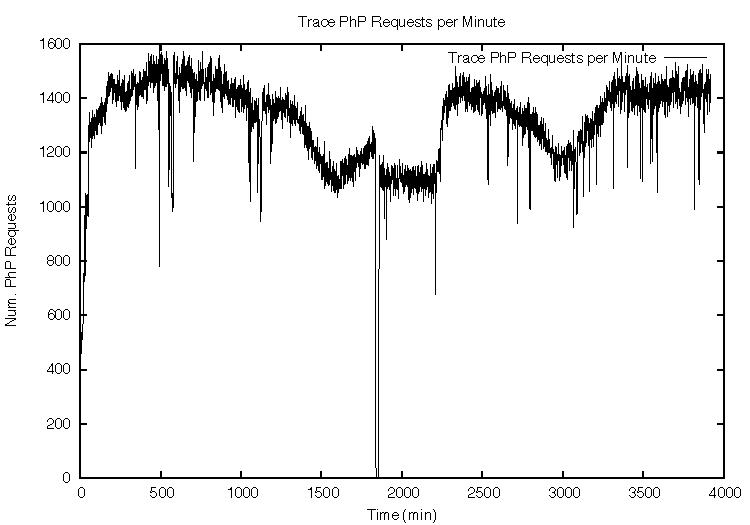
\includegraphics[width=0.49\textwidth, height=6cm]{./images/traceWorkload2011}
\end{center}
\vspace{-5mm}
\caption{Wikipedia trace workload.}
\label{workload}
\end{figure}

% Corina - I think this paragraph would be better suitable for future work:
%In addition, other properties may be also considered important when using the Wikipedia traces such as the interarrival time between requests, the distribution of page popularity, the mix of static/dynamic requests, the ratio of read/write operations and requests for non-existing pages and files.

%\begin{itemize}
%\item The intervarrival time between requests follows a Poisson distribution.

%\item The distribution of page popularity varies from very popular pages to those being accessed very infrequently.

%\item The mix of static/dynamic requests presents a strong variation. 

\begin{figure}
\begin{center}
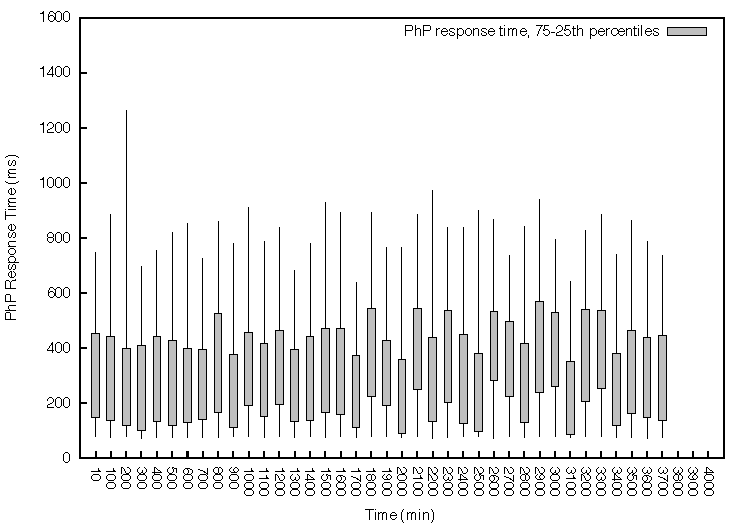
\includegraphics[width=0.49\textwidth, height=6cm]{./images/phpRespTimeDispersion2011}
\end{center}
\vspace{-5mm}
\caption{Complexity of PhP requests.}
\label{phpRespTimeDispersion}
\end{figure}

%\item The ratio of read/write operations vary having more reads than editions or creations of wiki pages.

%\begin{figure}
%\begin{center}
%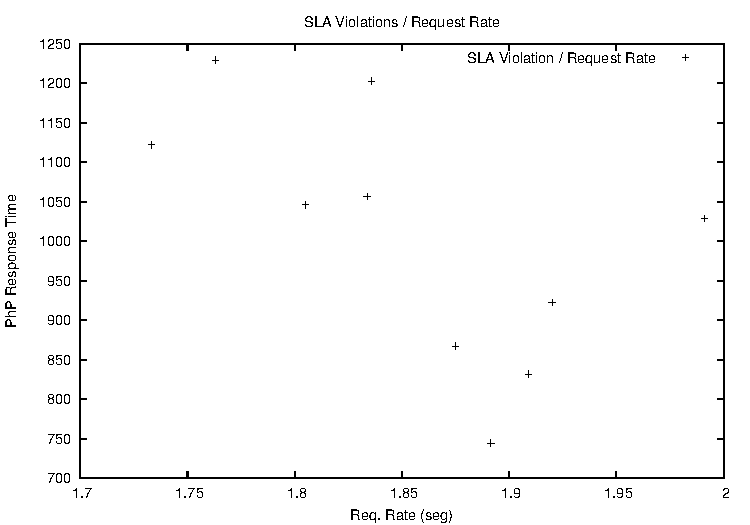
\includegraphics[width=0.49\textwidth, height=6cm]{./images/staticProv_reqRate}
%\end{center}
%\caption{Response time vs request rate.}
%\label{reqRate}
%\end{figure}

%\item A considerable amount of requests for non-existing pages and files add realism to the traffic.

%\end{itemize}


%By using real world server side software and data, we think the WikiBench benchmarking suite is a very  realistic and extensible research tool.

% these traces create workloads for WikiBench instead of creating purely synthetic workloads like other benchmarking tools have done.

%The workload-mix and the variable amount of data and visitors make of Wikipedia a valid example of elastic web application. In this paper, we focus in the scalability of the PhP web hosting service, and thereby as the number of PhP servers hosting MediaWiki scale out or back based on the demanding workload.

